\section{Introduction}
Part of the work carried out at Oversonic Robotics was the development of a simulator and testing platform.
The simulator, described in section \ref{section:sim}, is primarily intended to be a safe and reliable test environment where the new navigation algorithms can be tested. It is not intended to have a 1:1 simulation with the real robot, which is outside the scope of this thesis. 
As already mentioned, building robots means dealing with both the software and hardware side, the two components are inseparable and one does not exist without the other.
Dealing with the hardware part of the robot is a source of danger for people and the environment as software bugs can cause damage. In addition, testing a robot's behaviour in real life, the results of which are unknown, can cause mechanical damage and consequently much time would be lost in repair. Another not inconsiderable motivation lies in the wear and tear of the robot and its components: the batteries, for example, have a predefined life cycle and must be recharged in any case.
All these reasons support the development of a simulated environment to test new developments before implementing them on the real robot.
The testing module, described in section \ref{section:test}, addresses the need to have an indication of navigation performance. This need comes both from within the company, where it is important to evaluate how developments are improving it, and from outside, where the various stakeholders and customers can evaluate the project and understand how they can exploit the technology developed by Oversonic.
Not only this, as reported by \citet{Dhillon1991}, among the many types of tests, two of them are significant:
\begin{itemize}
    \item Reliability: obtain knowledge of failure occurrence patterns
    \item Performance: building reliable indicators on performance status
\end{itemize}
Tests are  moreover meant to have the following features:
\begin{itemize}
    \item Accuracy: whether the test can actually measure what it sets out to measure
    \item Resolution: how precisely it measures the proposed feature
    \item Repeatability: how repeatable it is, so that test performed over time are comparable 
\end{itemize}

\section{Simulator}
\label{section:sim}
\subsection{Introduction}
As already mentioned, the development of this simulator meets the practical need to be able to test new navigation algorithms in a safe manner. Given this need, the choice of simulation engine fell on Gazebo. The reasons behind this choice are many: Gazebo provides seamless integration with ROS and Rviz, and allows the working environment to be customised to the maximum, creating its own model of the robot, motors and sensors. On the other hand, this great freedom that is granted requires just as much expertise and an analytical study of the robot model. The approach we decided to follow was to first familiarise ourselves with the creation of three-dimensional models in URDF and XACRO by developing simple robot models and then adding sensors, as to make the model more articulated. Once familiar with the development environment, it was decided to create a model as faithful as possible to the R007 robot, combined with a differential drive base. 
\subsection{3D Model Creation}
The designed robot is made up of the following components:
\begin{itemize}
    \item a core box, representing the structure of the robot
    \item two-wheel drive, one on the right and one on the left side 
    \item two caster wheels, one in the front and one in the back. They are completely passive and the provide robot stability
    \item two Lidars, one place on the front and one on the back of the robot
\end{itemize}
First of all it is necessary to define the physical dimensions of the robot e.g. base dimensions, wheel parameters.
It is also necessary to specify the inertia values for every mass component existing: the core of the robot, the wheels and the caster wheels.
% \begin{minted}[fontsize={\fontsize{10}{11}\selectfont}]{xml}
% <robot name="gbot" xmlns:xacro="https://www.ros.org/wiki/xacro" >
%   <xacro:macro name="box_inertia" params="m w h d">
%     <inertial>
%       <mass value="${m}"/>
%       <inertia ixx="${m / 12.0 * (d*d + h*h)}" ixy="0.0" ixz="0.0"
%       iyy="${m / 12.0 * (w*w + h*h)}" iyz="0.0" izz="${m / 12.0 * (w*w + d*d)}"/>
%     </inertial>
%   </xacro:macro>
%   <xacro:macro name="cylinder_inertia" params="m r h">
%     <inertial>
%       <mass value="${m}"/>
%       <inertia ixx="${m*(3*r*r+h*h)/12}" ixy = "0" ixz = "0" iyy="${m*(3*r*r+h*h)/12}" 
%       iyz = "0" izz="${m*r*r/2}"/>
%     </inertial>
%   </xacro:macro>
%   <xacro:macro name="sphere_inertia" params="m r">
%     <inertial>
%       <mass value="${m}"/>
%       <inertia ixx="${2.0*m*(r*r)/5.0}" ixy="0.0" ixz="0.0" iyy="${2.0*m*(r*r)/5.0}"
%       iyz="0.0" izz="${2.0*m*(r*r)/5.0}"/>
%     </inertial>
%   </xacro:macro>
% </robot>
% \end{minted}
A robot can be described as having a number of link components and a number of joint elements that connect the links. The link element describes a stiff body with collision characteristics, visual characteristics (specifying the shape of the object for visualization purposes), and inertia.

The links used in this model were:
\begin{itemize}
    \item Robot core: base link and dummy link
    \item Wheels: right and left wheel
    \item Caster wheels: right and left caster wheel
    \item Lidar: front and back lidar
\end{itemize}
\begin{figure}[H]
    \centering
    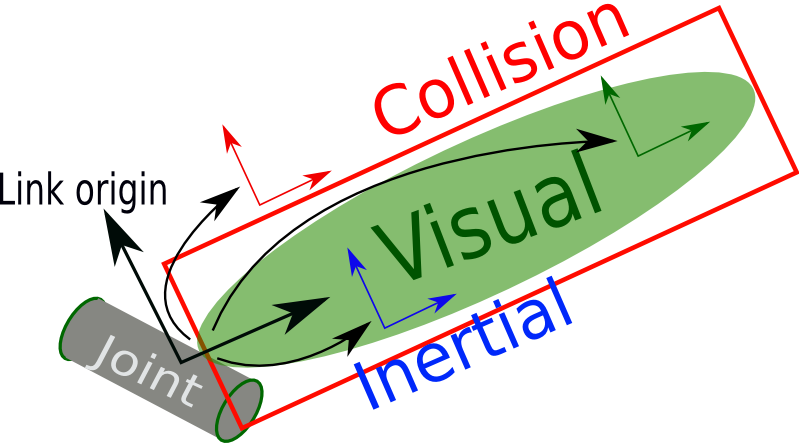
\includegraphics[scale=1.3]{Images/Chapter 5/inertial.png}
    \caption{Link representation that better explains the concepts of collision and visual}
    \label{fig:link}
\end{figure}
\begin{figure}[H]
    \centering
    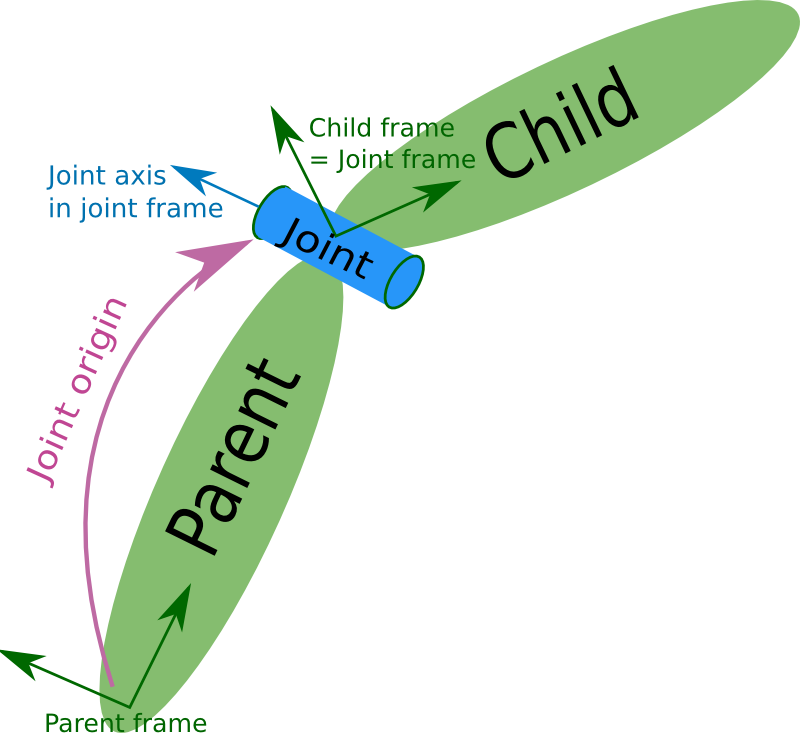
\includegraphics[scale=0.25]{Images/Chapter 5/joint.png}
    \caption{Joint visual representation}
    \label{fig:joint}
\end{figure}

% Hereafter is described the link for the box that was divided into a dummy link \texttt{base\_link} and a \texttt{chassis}:

% \begin{minted}[fontsize={\fontsize{10}{11}\selectfont}]{xml}
% <link name="base_link">
%     <visual>
%       <origin xyz="0 0 0" rpy="0 0 0"/>
%         <geometry>
%           <box size="0.001 0.001 0.001" />
%         </geometry>
%     </visual>
% </link>

% <link name="chassis">
%     <xacro:box_inertia m="10" w="${base_width}" h="${base_height}" d="${base_length}"/>
%     <collision>
%       <origin xyz="0 0 ${base_height/2}" rpy="0 0 0"/>
%       <geometry>
%         <box size="${base_length} ${base_width} ${base_height}"/>
%       </geometry>
%     </collision>
%     <visual>
%       <origin xyz="0 0 ${base_height/2}" rpy="0 0 0"/>
%       <geometry>
%         <box size="${base_length} ${base_width} ${base_height}"/>
%       </geometry>
%       <material name="water"/>
%     </visual>
%  </link>
% \end{minted}
The joint element sets the joint's safety restrictions and explains the kinematics and dynamics of the joint. There exists several types of joint, but in this specific application continuous joint was used for the casters and wheels,  whereas fixed joint for the robot core and Lidar were used.  Because it cannot move, a fixed joint is not really a joint: every level of freedom is locked. Continuous hinge joints have no upper or lower limitations and rotate about their axes, in this case particular attention must be paid to the collision parameters: friction has to be properly calibrated in the case of caster wheels, since a wrong friction or slip coefficient impedes the robot to turn properly. Since this simulator is not intended to be a 1:1 with the movements performed by the real robot, still we do not want friction to constrain movements, slip coefficient has been set to 1 whereas friction coefficient to 0. This choice has been made by trial and error, since by modifying those values, the robot could not follow the planner trajectories, leading to continuous drift.

% \begin{minted}[fontsize={\fontsize{10}{11}\selectfont}]{xml}
% <joint name="base_link_joint" type="fixed">
%     <origin xyz="0 0 ${wheel_radius}" rpy="0 0 0" />
%     <parent link="base_link"/>
%     <child link="chassis"/>
%   </joint>
% <joint name="${prefix}_wheel_joint" type="continuous">
%       <origin xyz="0 ${((wheel_separation/2))*reflect} 0"
%       rpy="0 0 0"/>
%       <parent link="chassis"/>
%       <child link="${prefix}_wheel"/>
%       <axis xyz="0 1 0"/>
% </joint>
% </xacro:macro>

% <joint name="${prefix}_caster_wheel_joint" type="continuous">
%       <axis xyz="1 1 1"/>
%       <parent link="chassis"/>
%       <child link="${prefix}_caster_wheel"/>
%       <origin xyz="${reflect*caster_wheel_joint_offset} 0 ${-wheel_radius+caster_wheel_radius}"
%       rpy="0 0 0"/>
% </joint>
% </xacro:macro>
% \end{minted}  

\begin{figure}[H]
\centering
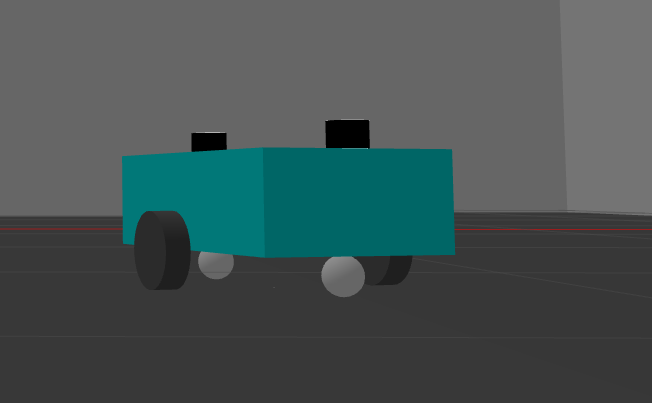
\includegraphics[scale = 0.5]{Images/Chapter 5/sim_3.png}
\caption{Robot model visualization}
\end{figure}

The complete code that builds the model up can be found at Appendix \ref{ch:appA}.
% The overall Rqt graph is: 
% \begin{figure}[H]
%     \centering
%     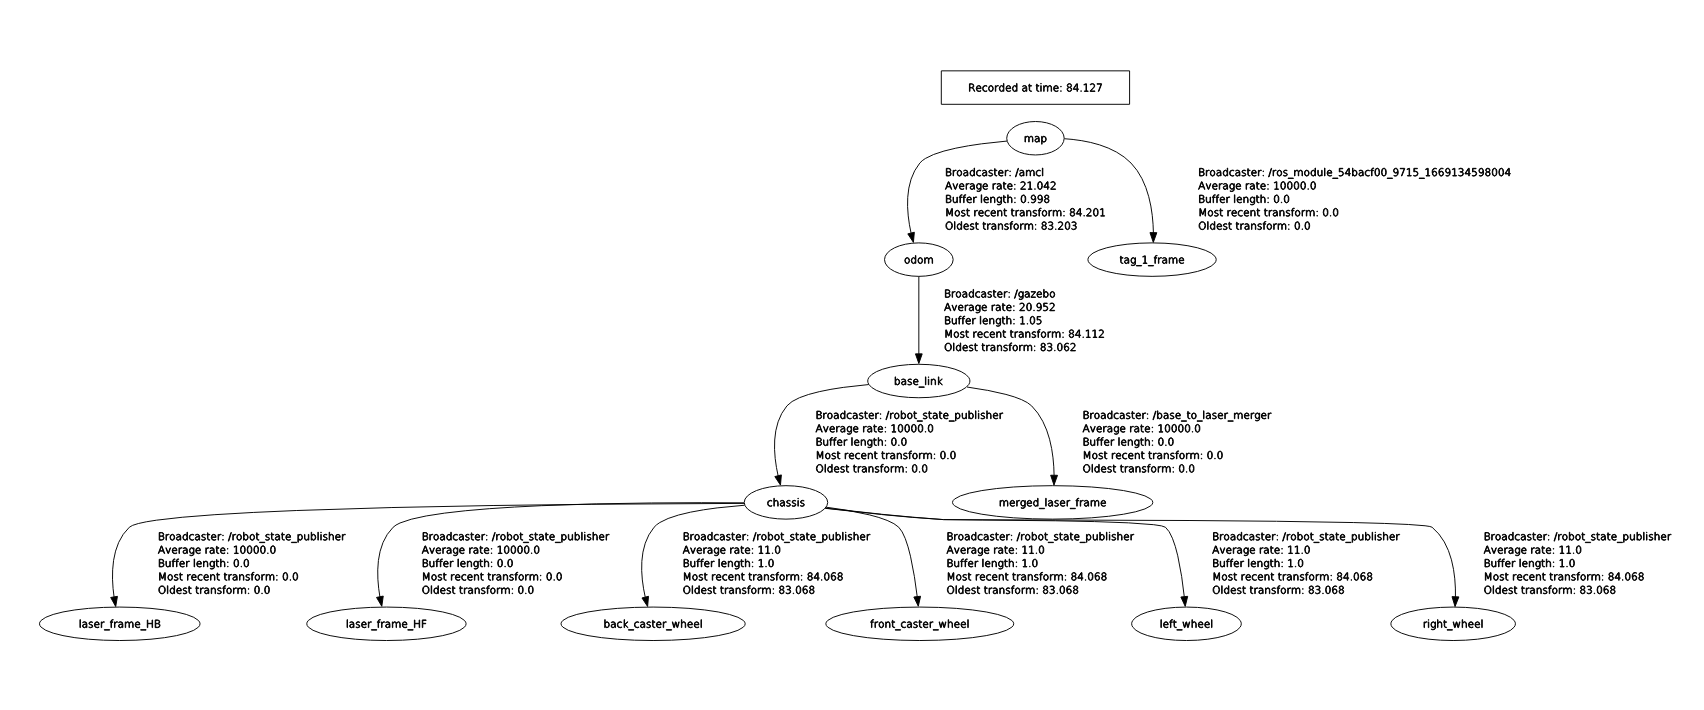
\includegraphics[scale=0.31]{Images/Chapter 5/rqt_graph_sim.png}
%     \caption{Rqt graph from the simulated robot}
%     \label{fig:rqt_graph_sim}
% \end{figure}
\subsection{Gazebo Plugins}
The strategy up to this point has been to create the 3D model of the robot, then specify the components and their dimensions, links and joint types. At this point the model is created but is no more than a mesh and cannot be used in navigation. In order to get the robot on track, it is necessary to duly integrate the model with a drive system, which mimics the physical motors, and lidar sensors. 
Gazebo provides plug-ins that meet this requirement. Two main plug-ins were used within the simulator: the differential\_drive\_controller for differential driving and the head\_hokuyo\_controller for lidar. 
In order to have the differential drive plug in working, a number of parameters must be set to bind it to the created XACRO model and to the already existing navigation stack. In particular, the plug-in needs to know the dimensions of the wheels and the joints to which they are connected, as well as the link of the robot body and the odometry topic. The speed command is acquired directly from the topic /twist\_mux/cmd\_vel, which is also used in the real robot. It is then necessary to specify the torque to be applied and the update rate. 
A similar argument must be made for the integration of the lidar sensor plug-in. It is necessary to specify all the topics that are normally used in the real robot to build a bridge between the simulated environment and the navigation stack. In particular, the topics used are /scanHF and /scanHB. It is also appropriate to modify the specifications of the simulated sensor to match those of YDlidar G4.
In addition, the plug-in for the d455 camera and the t265 camera can also be imported. The simulated depth camera can be used for the recognition of tags placed in the virtual environment as well as for pointcloud generation. The simulated tracking camera, on the other hand, is used for visual odometry by replacing the default odometry source parameter of the differential drive with the topic of the tracking camera.

\subsection{Virtual Environment}
The next step was to create a virtual environment where the robot can move and where the navigation algorithms can be tested. The approach used was to replicate the Oversonic Robotics development space. After acquiring the measurements of the real environment with laser metre, the 1:1 scale measurements were transported to the Gazebo environment. Gazebo in fact allows the creation of rooms from scratch, building walls and doors with centimetre-accurate measurements.
It also allows the insertion of obstacles and fiducial tags in the space.  
\begin{figure}[H]
\centering
\begin{tabular}{cc}
\subfloat[Bird's eye view of the virtual environment]{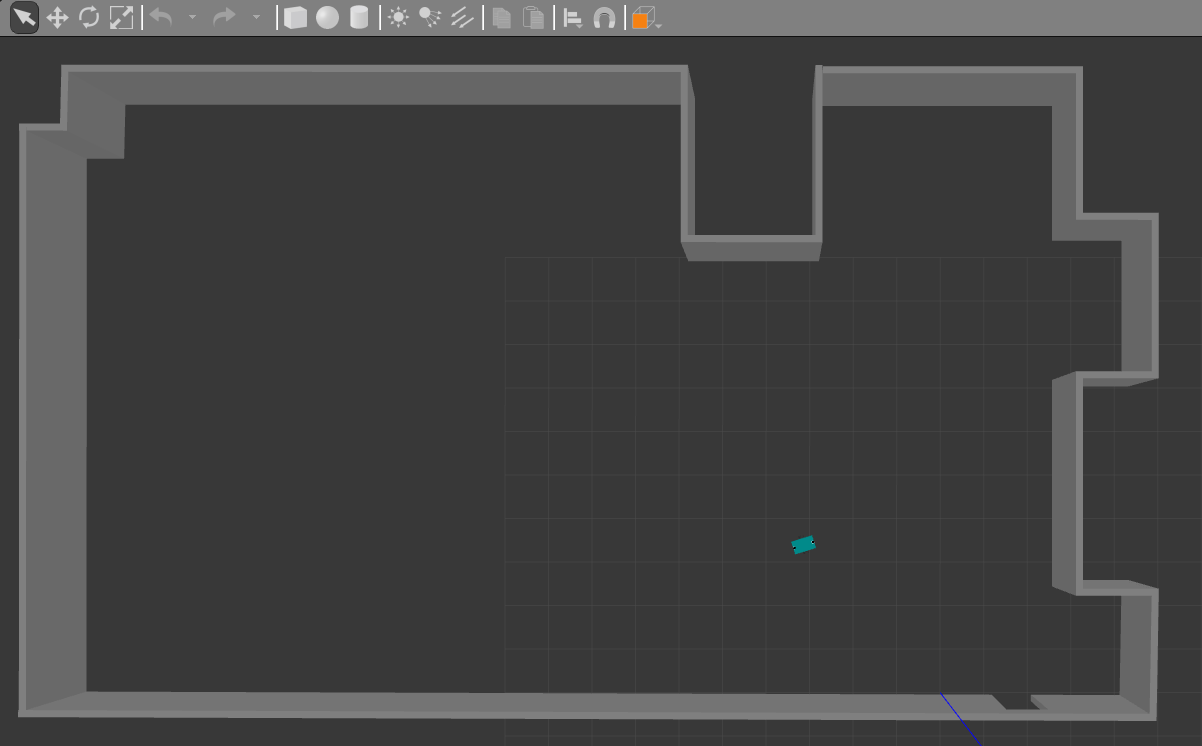
\includegraphics[scale = 0.18]{Images/Chapter 5/sim_sky_view.png}}&
\subfloat[Apriltag integration]{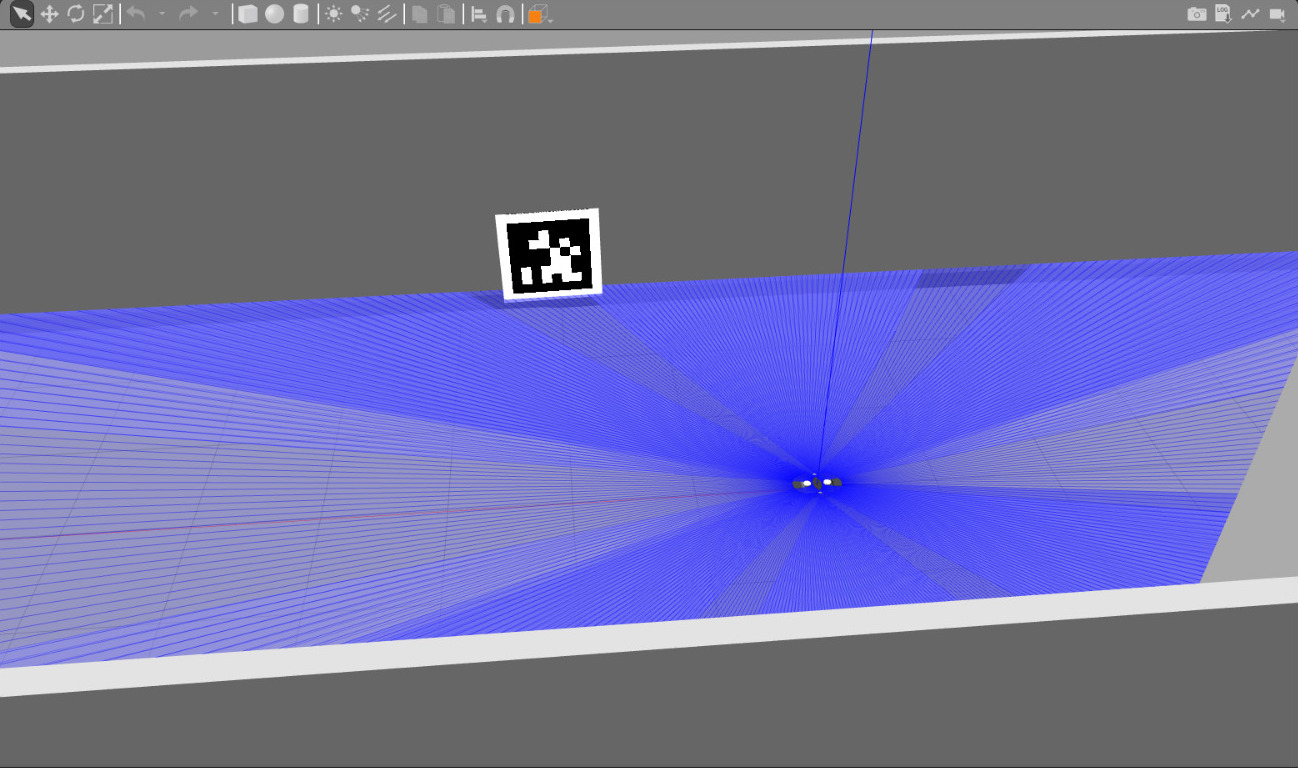
\includegraphics[scale=0.73]{Images/Chapter 5/sim6.jpeg}}\\
\end{tabular}
\caption{Production room simulated environment}
\label{fig:sim_obst_avoid}
\end{figure}
\subsection{Mapping and Navigating}
After constructing the virtual environment, the mapping of the new space is required. A launcher must then be set up to run all the simulation components created. Within the launch file, the newly created simulated world, the robot model with the required plug-ins and an Rviz spawner will be imported. Similar to what happens in the real world, we proceed to move the robot with the joystick and the SLAM toolbox takes care of creating a map. 
Once the map is obtained and cleared, the robot's navigation module can be tested. 
In figure \ref{fig:sim_obst_avoid} is reported an example of obstacle avoidance performed by the simulated robot. 

\begin{figure}[H]
\centering
\begin{tabular}{cc}
\subfloat[]{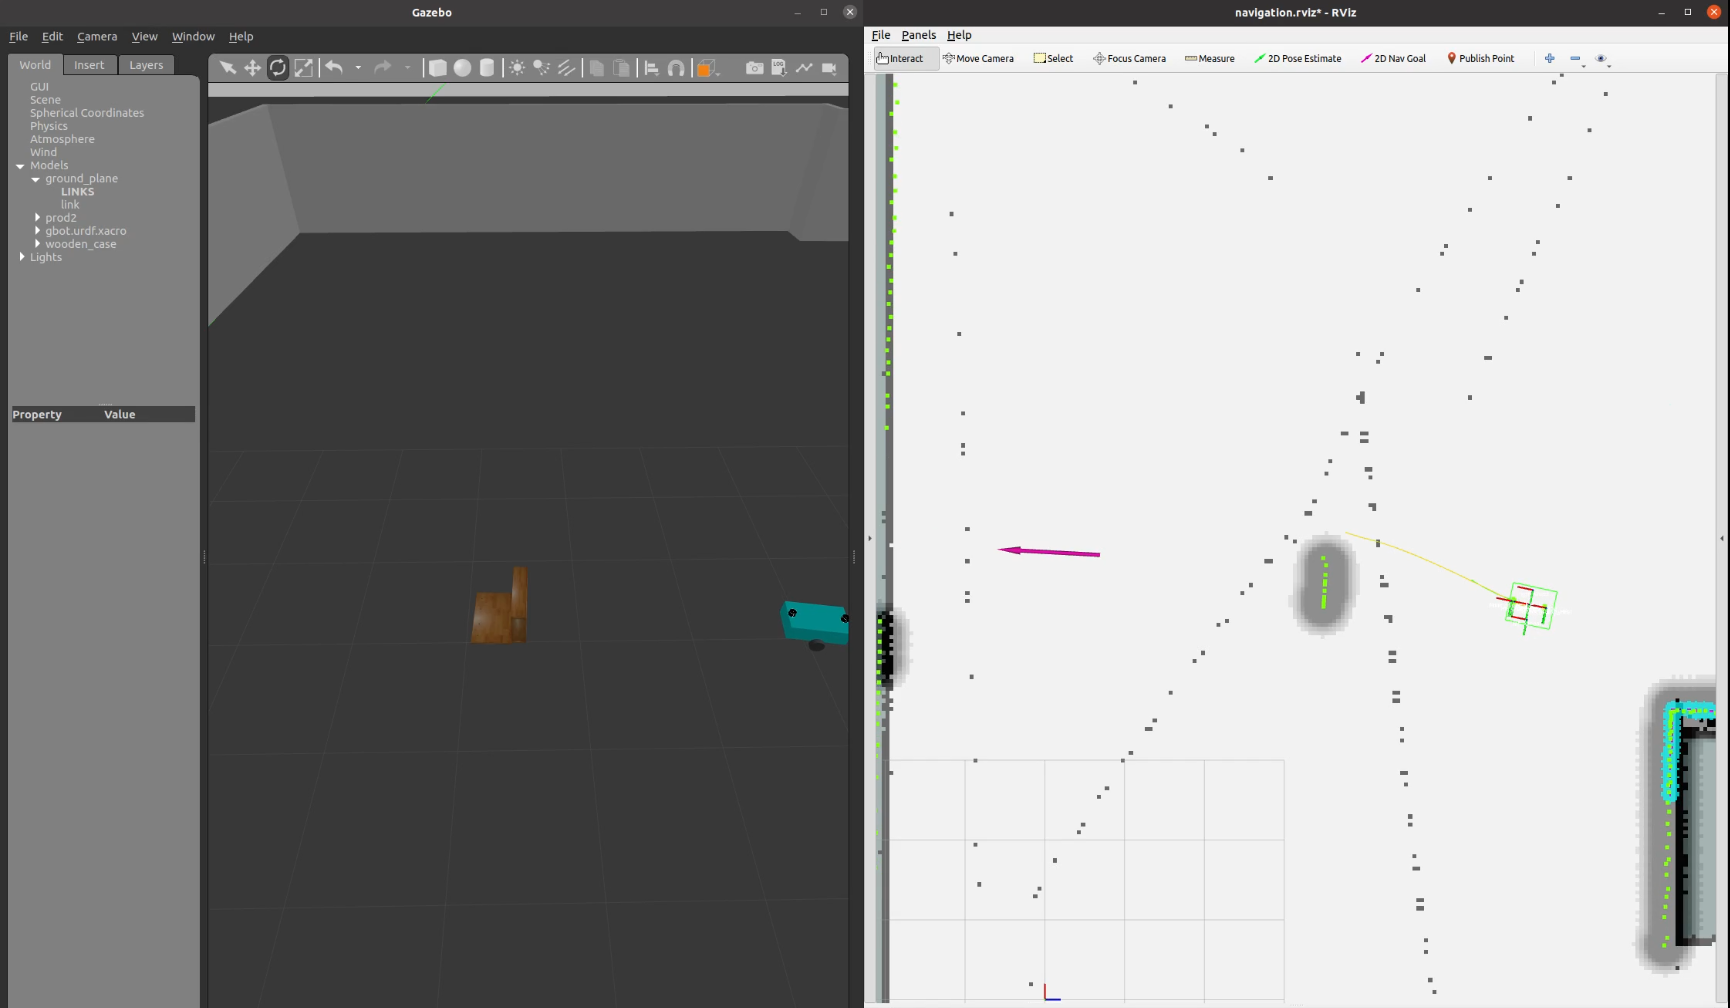
\includegraphics[width = 3.5in]{Images/Chapter 5/obstavoid2_1.png}}&
\subfloat[]{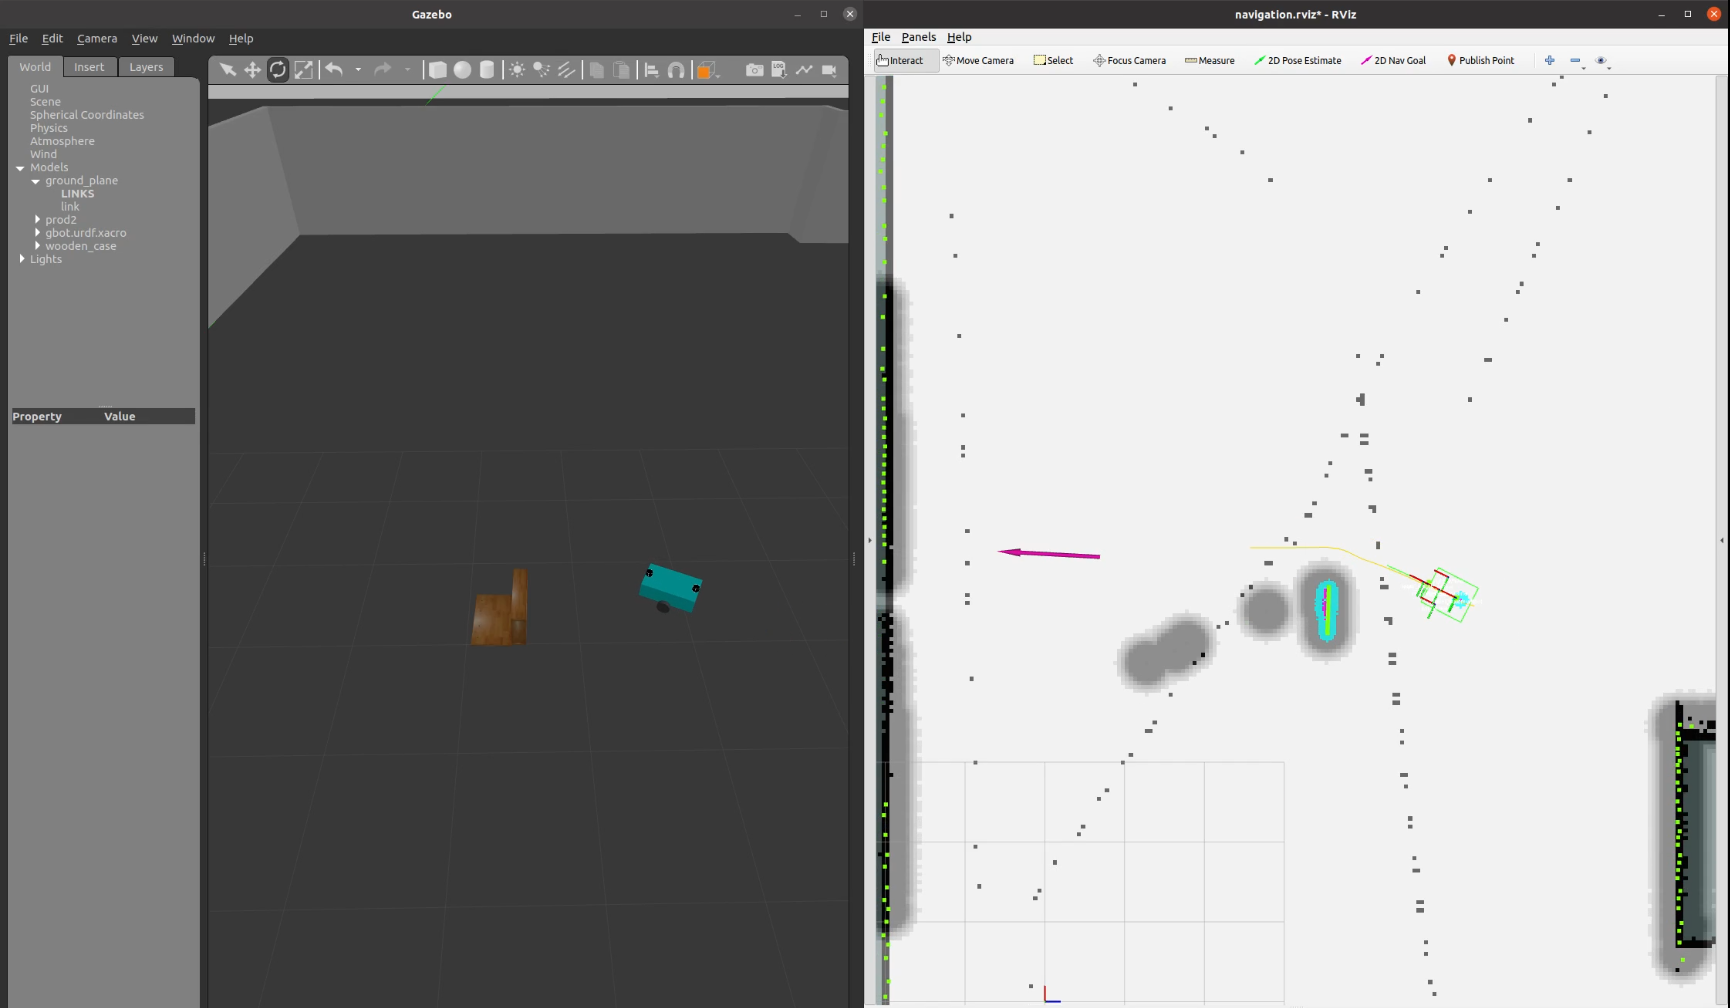
\includegraphics[width = 3.5in]{Images/Chapter 5/obstavoid2_2.png}}\\
\subfloat[]{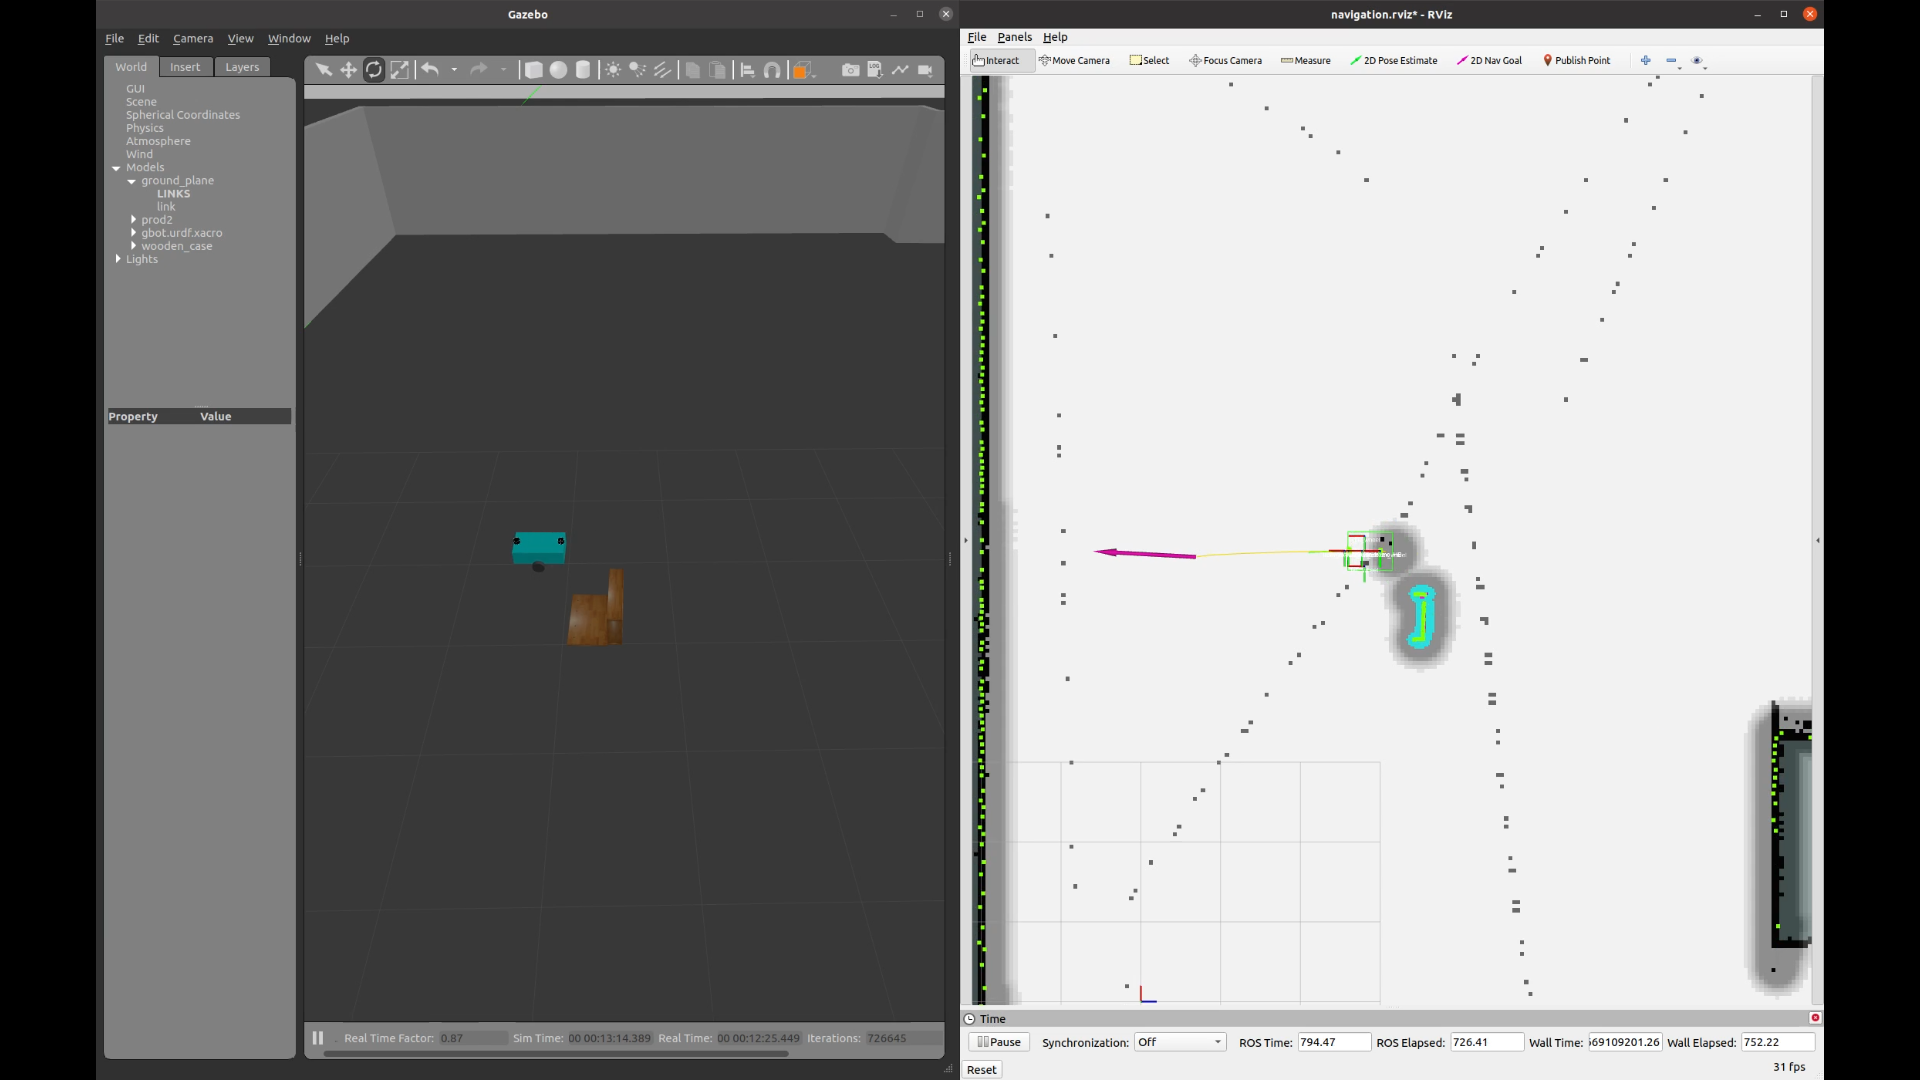
\includegraphics[width = 3.5in]{Images/Chapter 5/obstavoid2_4.png}}&
\subfloat[]{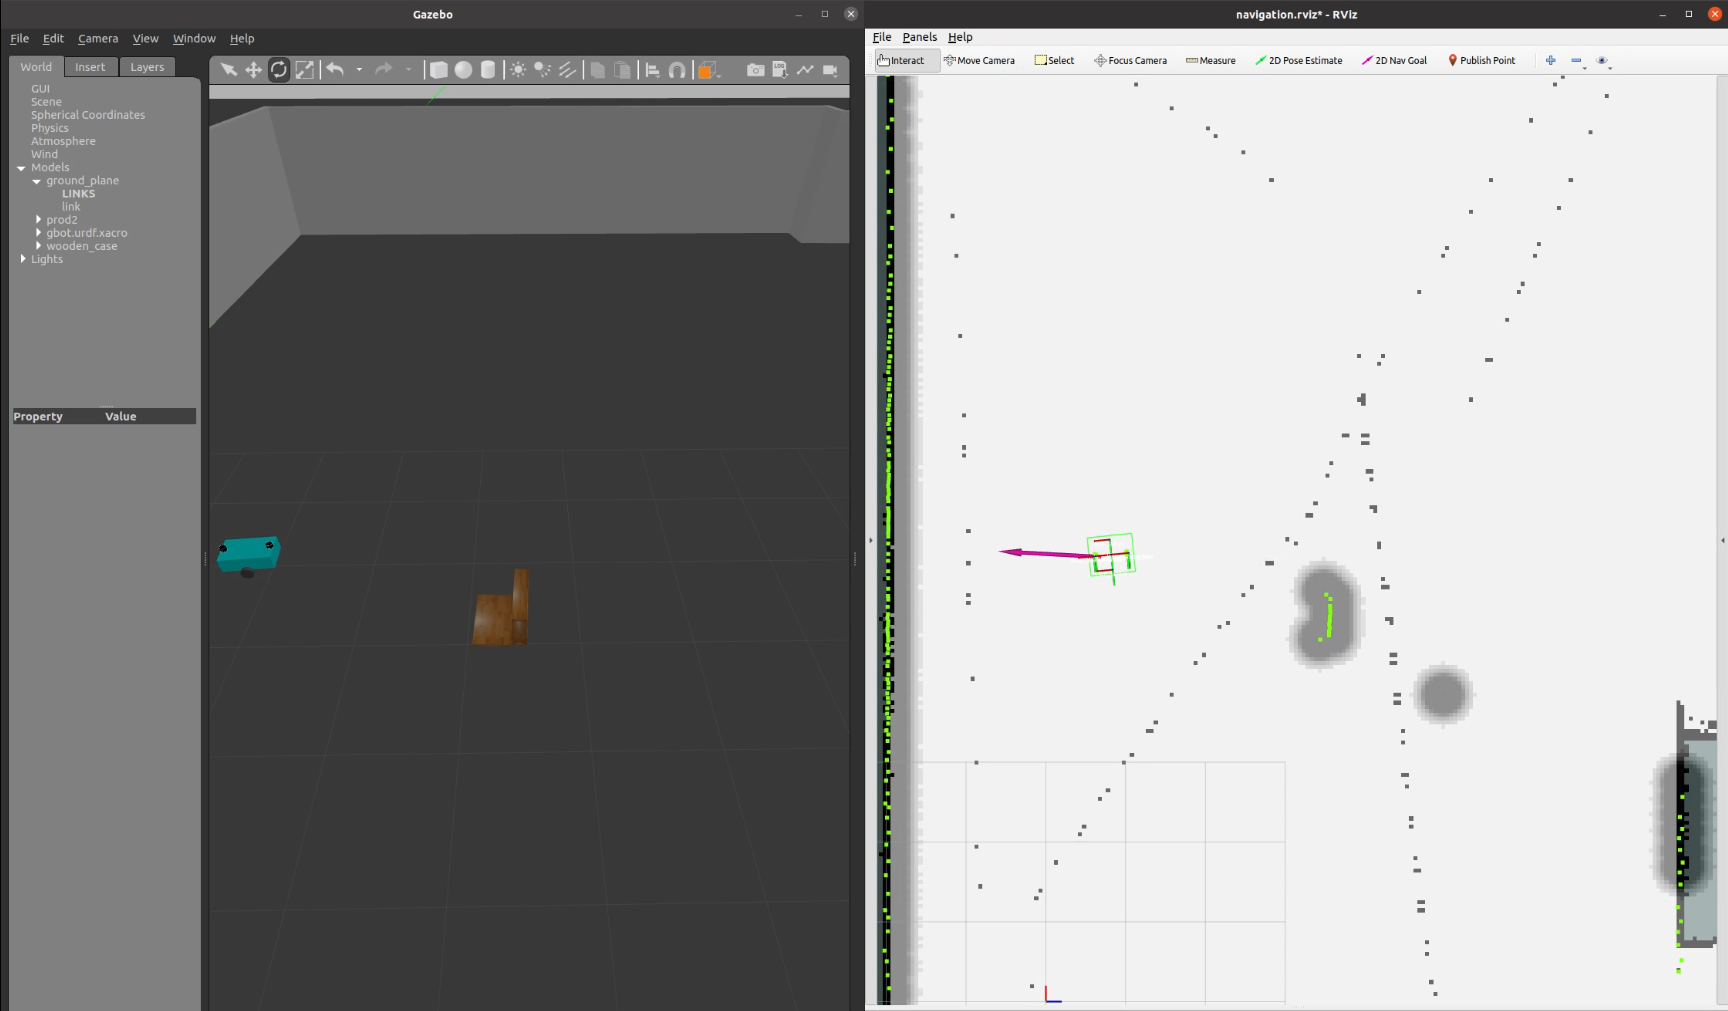
\includegraphics[width = 3.5in]{Images/Chapter 5/obstavoid2_3.png}}
\end{tabular}
\caption{Simulation of an obstacle avoidance movement}
\label{fig:sim_obst_avoid}
\end{figure}

\section{Testing Module}
\label{section:test}
The test module is designed to be a highly autonomous instrument where the operator only needs to indirectly monitor its progress.
To this end, the module was developed in Python, supplementing the original navigation stack with a part dedicated to plotting the route in real time and calculating statistics.
Starting from an unknown work are, the steps to be followed are as follows:
\begin{enumerate}
    \item Build the map of the environment (using SLAM toolbox), clean it from anomalies and load it on Oversonic database
    \item Design the path the robot is going to follow during its tests: the  path has to respond to specific behaviors we want to test, e.g. relocation via Apriltag, climbing a ramp, navigate close to walls and obstacles.
    Specify the starting position, a list of waypoints and a goal point, building a json file with their coordinates and uploading it to database
    \item Decide robot's configuration and the number of repetitions for the test
\end{enumerate}
Oversonic adopts waypoint logic for its navigation tasks: waypoint navigation is a commonly used approach in mobile robots navigation.
When the robot has to perform predefined path (for example in testing framework, as this thesis is) it is convenient to specify some points between its starting and arriving point where the robot has to pass by or near by.  
In the scope of this thesis, a  new waypoint is sent as a goal to the robot when at a distance of less than one metre from the last received waypoint.
Clearly, tests are significant only if repeated for a high number of times so that meaningful statistics are set up.
Test pattern is thus set up via Oversonic's interface where it is possible to load test configuration:
\begin{itemize}
    \item Robot: which robot is going to perform the movement
    \item Map: where the robot will be moving
    \item Mission: the path it is going to run
    \item Repetitions: how many times should the mission iterates
\end{itemize}

Once the configurations are set, the interface lets the test responsible to select the number of repetitions the robot is going to perform.

\subsection{Performance Measurement Definition}
\label{subsection:performancedef}
As introduce, tests need to be accurate, resolute and repeatable. For the purpose of performance measurement, the  following values of interest are given for each measurement configuration: 
\begin{itemize}
    \item AVG SPEED: average speed over the entire path [m/s]
    \item FW AVG SPEED: average speed while navigating (its the avg speed from which we exclude on-site rotations) [m/s]
    \item ROT AVG SPEED: rotational average speed [rad/s]
    \item NAV DISTANCE: total distance calculated by odometry [m] \item TOP SPEED: top speed recorded [m/s]
    \item NAV TIME: total time spent [s] 
    \item FW MOVING TIME: moving forward time [s]
    \item ROTATING TIME: time the robot spends rotating in place [s]
    \item OBSTACLES: number of obstacles on the path [-]
\end{itemize}

The Navigation Performance index, also known as NP, is a metrics that returns the goodness of the navigation for a set of measurements. It has been developed to provide a summary indicator of performance at a glance. 
\begin{equation}
        NP = W * X =
    \begin{bmatrix}
            w_{1} & w_{2} & w_{3} & w_{4}
    \end{bmatrix}
    \begin{bmatrix}
        & x_{1} &\\
        & x_{2} &\\
        & x_{3} &\\
        & x_{4} &\\
    \end{bmatrix}
\end{equation}
The formula is defined by the vector product of the row vector W with column vector X.
X gathers four states measurements:
\begin{equation}
    x_{1} = \frac{Navigated Distance}{Path Distance}
\end{equation}
\begin{equation}
    x_{2} = \frac{Forward Average Speed}{Requested Speed}
\end{equation}
\begin{equation}
    x_{3} = \frac{ Moving Fw Time}{ Navigation Time}
\end{equation}
\begin{equation}
    x_{4} = \texttt{min}(OBSTACLES*0.25;1)
\end{equation}
whereas W is a vector that is used to weight the states on the overall performance. The values of the weights have been chosen trying to penalize blocking movements and trying to promote the ones that keeps the robot forward speed high.
\begin{equation}
    W = 
    \begin{bmatrix}
        25 & 25 & 30 & 20
    \end{bmatrix}
\end{equation}
Overall the NP index has the following formulation:
\begin{equation}
    NP = \frac{w_{1}*x_{1}+w_{2}*x_{2}+w_{3}*x_{3}+w_{4}*x_{4} }{w_{1} + w_{2} + w_{3} + w_{4}} 
    = \frac{15*x_{1}+30*x_{2}+25*x_{3}+30*x_{4}}{100}
\end{equation}


\subsection{Code Explanation}
The testing module is based on a callback structure. A ROS node called 'measures' is initialised and subscribed to three topics: goal\_status, cmd\_vel\_mux\_out and odom. 
We begin by explaining the concept of goal\_status. In fact, it is necessary to know what status the robot is in in order to distinguish the various phases and obtain reliable statistics. 
The built in class of Oversonic \texttt{goal\_status} arbitrates the management of statuses in a tree structure and decides to send the global status to the mission service. A global status, called goal\_status arbitrates two sub-states: move\_base\_flex and motion\_status 
Move\_base\_flex is provided by move\_base package and handles the statuses as:
\begin{itemize}
    \item Pending         = 0
    \item Active          = 1
    \item Preempted      = 2
    \item Succeeded       = 3
    \item Aborted         = 4
    \item Rejected        = 5
    \item Preempting      = 6
    \item Recalling       = 7
    \item Recalled        = 8
    \item Lost            = 9
\end{itemize}
The motion\_status is still an enumerate and takes the same states as the move\_base. Arbitrage checks the statuses and the last updated one, if coincident, is sent to the mission service. 
For proper test handling, a subclass, called rel\_movement\_status, was then implemented. 
The states are defined as: 
\begin{itemize}
    \item Not started = 0
    \item Navigating = 1
    \item Rotating = 2
    \item Reversing = 3
    \item Stuck = 4
\end{itemize}
This class monitors the robot's movements and understands if it is advancing, rotating or if it is stuck. The status provided does not enter into the arbitration mentioned above, but is simply an aid to the collection of measurement data and does not communicate with the mission service.
Only when both statuses are completed does the global status send the mission completion signal to the mission service via an MQTT message dispatcher. 
Cmd\_vel\_mux is a topic that exchanges messages regarding the velocity command: a multiplexer for command velocity inputs. Arbitrates incoming cmd\_vel messages from several topics, allowing one topic at a time to command the robot, based on priorities. It also dislocates current allowed topic if no messages are received after a configured timeout. All topics, together with their priority and timeout are configured through a YAML file. In our case, the two topics entering the mux are: the autonomous navigation cmd\_vel and the joystick steering cmd\_vel. The yaml file has been configured to give priority to joystick control. The last topic is odom and simply provides the message regarding odometry.
At this point, the three topics are used within a callback where each time they communicate a message, data is collected and used to calculate statistics. The programme handles the logic through a while loop that remains active until ROS is active or, more selectively, until the goal status is succeeded.
Specifically the module not only provides overall statistics but also compute performance intra waypoints. This feature was introduced in order to get a better glance of where the robot suffered from issues or where navigation speed decreased. This was possible by managing goal status in a different manner: waypoints are sent to the robot via a MQTT message and a new waypoint is sent to the robot only when it arrives around a waypoint with customisable accuracy. So every time a new waypoint is delivered to the system, statistics are computed and saved. When eventually the robot reaches the goal, the overall statistics for the lap are computed and saved into a separated xls file.
The files are saved in subfolder of the navigation module, called \texttt{Datasheets}, where two files are initialized (if not already existing): 
\begin{itemize}
    \item \texttt{Waypoints.xls}: statistics of intra waypoints performance are saved. Three relevant metrics are chosen (Distance travelled, Time spent and Average Speed) and each data row corresponds to an intra waypoint measurement. After reaching the goal, the programm splits the set of measurements by inserting an end row. 
    \item\texttt{Measurements.xls}: relevant metrics per lap are saved in each row, where column performance indicators are as defined in subsection \ref{subsection:performancedef}.
\end{itemize}
    
The full description of the python code and for a detailed breakdown of how statistics are computed refer to Appendix \ref{ch:appB}.
    
\subsection{Test Case}

The route created involves a path of approximately 25 m that involved passing through a 1 m wide doorway. The plot in figure \ref{fig: test_map} is obtained through the designed plotter.
The automatic relocation algorithm using fiducial tags of known position on the map is also tested. 
There are no fixed or moving obstacles other than those already mapped in order to take a snapshot of the current status and robustness of navigation under 'stable' conditions 

\begin{figure}[H]
    \centering
    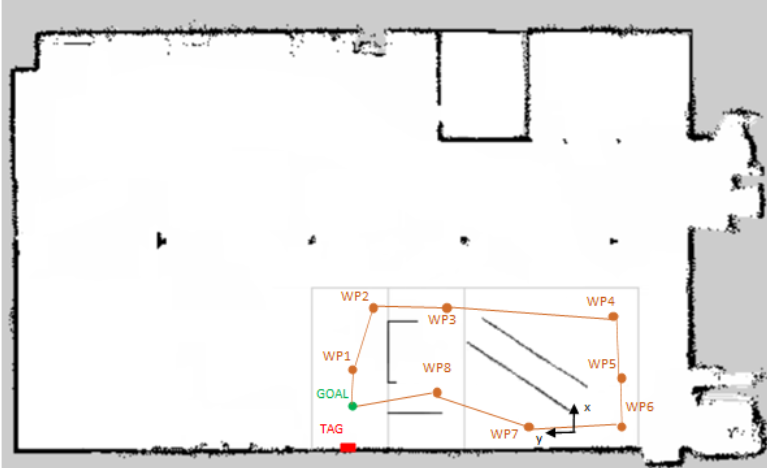
\includegraphics[scale=0.5]{Images/Chapter 5/testmap.png}
    \caption{Map visualization: theoretical path required. Total distance: 25.0 m}
    \label{fig: test_map}
\end{figure}

Below are defined the waypoints and the final goal. The assumption is that the starting point, also known as waypoint 0, coincides with the goal. This ensures test to iterate from itself in a loop of laps. 
\begin{table}[H]
\centering
\begin{tabular}{@{}|c|c|c|@{}}
\toprule
\textbf{\begin{tabular}[c]{@{}c@{}}Waypoint \\ Coordinate\end{tabular}} &
  \textbf{\begin{tabular}[c]{@{}c@{}}x\\ {[}m{]}\end{tabular}} &
  \textbf{\begin{tabular}[c]{@{}c@{}}y\\ {[}m{]}\end{tabular}} \\ \midrule
\textbf{WP1}  & 2.1  & 6.3  \\ \midrule
\textbf{WP2}  & 4.2  & 5.7  \\ \midrule
\textbf{WP3}  & 4.2  & 3.1  \\ \midrule
\textbf{WP4}  & 3.9  & -2.2 \\ \midrule
\textbf{WP5}  & 1.9  & -2.5 \\ \midrule
\textbf{WP6}  & -0.2 & -2.4 \\ \midrule
\textbf{WP7}  & 0.0  & 1    \\ \midrule
\textbf{WP8}  & 1.2  & 3.4  \\ \midrule
\textbf{GOAL} & 0.5  & 6.6  \\ \bottomrule
\end{tabular}
\caption{Waypoints and Goal coordinates}
\label{tab:waypoint}
\end{table}
% Please add the following required packages to your document preamble:
% \usepackage{booktabs}
% \usepackage{multirow}
\begin{table}[H]
\centering
\begin{tabular}{@{}|c|cc|@{}}
\toprule
\textbf{Settings}       & \multicolumn{2}{c|}{\textbf{Robot: R012}}                          \\ \midrule
\textbf{$\tau$ {[}-{]}} & \multicolumn{2}{c|}{5}                                             \\ \midrule
\multirow{3}{*}{\textbf{\begin{tabular}[c]{@{}c@{}}max. acc\\ {[}m/s\textasciicircum{}2{]}\end{tabular}}} & \multicolumn{1}{c|}{0.9} & at speed = 0.6 {[}m/s{]}         \\ \cmidrule(l){2-3} 
                        & \multicolumn{1}{c|}{1.0}  & at speed = 0.7 {[}m/s{]}               \\ \cmidrule(l){2-3} 
                        & \multicolumn{1}{c|}{1.05} & at speed = 0.8 {[}m/s{]}               \\ \midrule
\multirow{2}{*}{\textbf{slip {[}-{]}}}                                                                    & \multicolumn{1}{c|}{0.9} & if speed \textless {[}0.8 m/s{]} \\ \cmidrule(l){2-3} 
                        & \multicolumn{1}{c|}{0.8}  & if speed \textgreater{}= {[}0.8 m/s{]} \\ \bottomrule
\end{tabular}
\caption{Robot Configuration}
\label{tab:mech_set}
\end{table}

 

\subsection{Experimental Data and Results}
Tests were carried out at 3 different desired speeds (0.6, 0.7 and 0.8 m/s) in order to assess how the statistics varied as the required speed changed.
\subsubsection{Test Requested Speed at 0.6 m/s}

% Please add the following required packages to your document preamble:
% \usepackage{graphicx}
% \usepackage[table,xcdraw]{xcolor}
% If you use beamer only pass "xcolor=table" option, i.e. \documentclass[xcolor=table]{beamer}
\begin{table}[H]
\centering
\resizebox{\columnwidth}{!}{%
\begin{tabular}{lcccccccc}
\hline
\multicolumn{1}{|l}{} &
  \multicolumn{1}{c|}{\textbf{\begin{tabular}[c]{@{}c@{}}Avg Speed\\ {[}m/s{]}\end{tabular}}} &
  \multicolumn{1}{c|}{\textbf{\begin{tabular}[c]{@{}c@{}}Fw Avg  Speed\\ {[}m/s{]}\end{tabular}}} &
  \multicolumn{1}{c|}{\textbf{\begin{tabular}[c]{@{}c@{}}Rot avg speed\\ {[}rad/s{]}\end{tabular}}} &
  \multicolumn{1}{c|}{\textbf{\begin{tabular}[c]{@{}c@{}}Nav Dist\\ {[}m{]}\end{tabular}}} &
  \multicolumn{1}{c|}{\textbf{\begin{tabular}[c]{@{}c@{}}Top Speed\\ {[}m/s{]}\end{tabular}}} &
  \multicolumn{1}{c|}{\textbf{\begin{tabular}[c]{@{}c@{}}Nav Time\\ {[}s{]}\end{tabular}}} &
  \multicolumn{1}{c|}{\textbf{\begin{tabular}[c]{@{}c@{}}Moving Fw Time\\ {[}s{]}\end{tabular}}} &
  \multicolumn{1}{c|}{\textbf{\begin{tabular}[c]{@{}c@{}}Rotating Time\\ {[}s{]}\end{tabular}}} \\ \hline
\multicolumn{9}{|c|}{\textbf{Requested Speed = 0.6 {[}m/s{]}}} \\ \hline
\multicolumn{1}{|l|}{\textbf{AVG}} &
  \multicolumn{1}{c|}{{\color[HTML]{595959} 0,48}} &
  \multicolumn{1}{c|}{{\color[HTML]{595959} 0,54}} &
  \multicolumn{1}{c|}{{\color[HTML]{595959} 0,73}} &
  \multicolumn{1}{c|}{{\color[HTML]{595959} 25,00}} &
  \multicolumn{1}{c|}{{\color[HTML]{595959} 0,63}} &
  \multicolumn{1}{c|}{{\color[HTML]{595959} 52,73}} &
  \multicolumn{1}{c|}{{\color[HTML]{595959} 41,04}} &
  \multicolumn{1}{c|}{{\color[HTML]{595959} 6,31}} \\ \hline
\multicolumn{1}{|l|}{\textbf{MIN}} &
  \multicolumn{1}{c|}{{\color[HTML]{595959} 0,39}} &
  \multicolumn{1}{c|}{{\color[HTML]{595959} 0,52}} &
  \multicolumn{1}{c|}{{\color[HTML]{595959} 0,49}} &
  \multicolumn{1}{c|}{{\color[HTML]{595959} 24,69}} &
  \multicolumn{1}{c|}{{\color[HTML]{595959} 0,62}} &
  \multicolumn{1}{c|}{{\color[HTML]{595959} 49,89}} &
  \multicolumn{1}{c|}{{\color[HTML]{595959} 38,90}} &
  \multicolumn{1}{c|}{{\color[HTML]{595959} 4,52}} \\ \hline
\multicolumn{1}{|l|}{\textbf{MAX}} &
  \multicolumn{1}{c|}{{\color[HTML]{595959} 0,50}} &
  \multicolumn{1}{c|}{{\color[HTML]{595959} 0,55}} &
  \multicolumn{1}{c|}{{\color[HTML]{595959} 0,82}} &
  \multicolumn{1}{c|}{{\color[HTML]{595959} 25,57}} &
  \multicolumn{1}{c|}{{\color[HTML]{595959} 0,63}} &
  \multicolumn{1}{c|}{{\color[HTML]{595959} 64,69}} &
  \multicolumn{1}{c|}{{\color[HTML]{595959} 43,84}} &
  \multicolumn{1}{c|}{{\color[HTML]{595959} 14,91}} \\ \hline
\multicolumn{1}{|l|}{\textbf{VAR}} &
  \multicolumn{1}{c|}{{\color[HTML]{595959} 0,0015}} &
  \multicolumn{1}{c|}{{\color[HTML]{595959} 0,0001}} &
  \multicolumn{1}{c|}{{\color[HTML]{595959} 0,0121}} &
  \multicolumn{1}{c|}{{\color[HTML]{595959} 0,0883}} &
  \multicolumn{1}{c|}{{\color[HTML]{595959} 0,0000}} &
  \multicolumn{1}{c|}{{\color[HTML]{595959} 28,0762}} &
  \multicolumn{1}{c|}{{\color[HTML]{595959} 2,4016}} &
  \multicolumn{1}{c|}{{\color[HTML]{595959} 14,4604}} \\ \hline
\end{tabular}%
}
\caption{Statistics at 0.6 m/s}
\label{tab:speed06test}
\end{table}
Observing the data some useful insights can be extracted: the ratio total average speed to requested speed is equal to 79 \%, the ratio forward average speed to requested speed is equal to 91\%. The performance index suggests a NP value of 71 \%.
States measurements are evaluated as $x_1$ = 0.998, $x_2$ = 0.907, $x_3$ = 0.778 and $x_4$ = 0, since no obstacle was present.

\subsubsection{Test Requested Speed at 0.7 m/s}
Requested speed is increased by 16.7 \%.
The ratio total average speed to requested speed is increades up to 82 \%, the ratio forward average speed to requested speed is steady at 91\%. The performance index suggests a NP value of 73 \% as in the first case.
States measurements are evaluated as $x_1$ = 1.01, $x_2$ = 0.914, $x_3$ = 0.82 and $x_4$ = 0, since no obstacle was present. Increasing the speed leads to an increase in all of the performance states.
\begin{table}[H]
\centering
\resizebox{\columnwidth}{!}{%
\begin{tabular}{|lcccccccc|}
\hline
 &
  \multicolumn{1}{c|}{\textbf{\begin{tabular}[c]{@{}c@{}}Avg Speed\\ {[}m/s{]}\end{tabular}}} &
  \multicolumn{1}{c|}{\textbf{\begin{tabular}[c]{@{}c@{}}Fw Avg  Speed\\ {[}m/s{]}\end{tabular}}} &
  \multicolumn{1}{c|}{\textbf{\begin{tabular}[c]{@{}c@{}}Rot avg speed\\ {[}rad/s{]}\end{tabular}}} &
  \multicolumn{1}{c|}{\textbf{\begin{tabular}[c]{@{}c@{}}Nav Dist\\ {[}m{]}\end{tabular}}} &
  \multicolumn{1}{c|}{\textbf{\begin{tabular}[c]{@{}c@{}}Top Speed\\ {[}m/s{]}\end{tabular}}} &
  \multicolumn{1}{c|}{\textbf{\begin{tabular}[c]{@{}c@{}}Nav Time\\ {[}s{]}\end{tabular}}} &
  \multicolumn{1}{c|}{\textbf{\begin{tabular}[c]{@{}c@{}}Moving Fw Time\\ {[}s{]}\end{tabular}}} &
  \textbf{\begin{tabular}[c]{@{}c@{}}Rotating Time\\ {[}s{]}\end{tabular}} \\ \hline
\multicolumn{9}{|c|}{\textbf{Requested Speed = 0.7 {[}m/s{]}}} \\ \hline
\multicolumn{1}{|l|}{\textbf{AVG}} &
  \multicolumn{1}{c|}{{\color[HTML]{595959} 0,57}} &
  \multicolumn{1}{c|}{{\color[HTML]{595959} 0,64}} &
  \multicolumn{1}{c|}{{\color[HTML]{595959} 0,82}} &
  \multicolumn{1}{c|}{{\color[HTML]{595959} 25,29}} &
  \multicolumn{1}{c|}{{\color[HTML]{595959} 0,73}} &
  \multicolumn{1}{c|}{{\color[HTML]{595959} 44,01}} &
  \multicolumn{1}{c|}{{\color[HTML]{595959} 36,10}} &
  {\color[HTML]{595959} 3,96} \\ \hline
\multicolumn{1}{|l|}{\textbf{MIN}} &
  \multicolumn{1}{c|}{{\color[HTML]{595959} 0,56}} &
  \multicolumn{1}{c|}{{\color[HTML]{595959} 0,63}} &
  \multicolumn{1}{c|}{{\color[HTML]{595959} 0,70}} &
  \multicolumn{1}{c|}{{\color[HTML]{595959} 25,11}} &
  \multicolumn{1}{c|}{{\color[HTML]{595959} 0,72}} &
  \multicolumn{1}{c|}{{\color[HTML]{595959} 43,64}} &
  \multicolumn{1}{c|}{{\color[HTML]{595959} 34,20}} &
  {\color[HTML]{595959} 3,11} \\ \hline
\multicolumn{1}{|l|}{\textbf{MAX}} &
  \multicolumn{1}{c|}{{\color[HTML]{595959} 0,58}} &
  \multicolumn{1}{c|}{{\color[HTML]{595959} 0,65}} &
  \multicolumn{1}{c|}{{\color[HTML]{595959} 0,90}} &
  \multicolumn{1}{c|}{{\color[HTML]{595959} 25,42}} &
  \multicolumn{1}{c|}{{\color[HTML]{595959} 0,74}} &
  \multicolumn{1}{c|}{{\color[HTML]{595959} 44,59}} &
  \multicolumn{1}{c|}{{\color[HTML]{595959} 38,59}} &
  {\color[HTML]{595959} 4,82} \\ \hline
\multicolumn{1}{|l|}{\textbf{VAR}} &
  \multicolumn{1}{c|}{{\color[HTML]{595959} 0,000062}} &
  \multicolumn{1}{c|}{{\color[HTML]{595959} 0,000067}} &
  \multicolumn{1}{c|}{{\color[HTML]{595959} 0,004414}} &
  \multicolumn{1}{c|}{{\color[HTML]{595959} 0,017557}} &
  \multicolumn{1}{c|}{{\color[HTML]{595959} 0,000067}} &
  \multicolumn{1}{c|}{{\color[HTML]{595959} 0,091824}} &
  \multicolumn{1}{c|}{{\color[HTML]{595959} 1,954462}} &
  {\color[HTML]{595959} 0,287495} \\ \hline
\end{tabular}%
}
\caption{Statistics at 0.7 m/s}
\label{tab:speed07test}
\end{table}

\subsubsection{Test Requested Speed at 0.8 m/s}
Requested speed is increased by 14.3 \%.
The ratio total average speed to requested speed decreases to 80 \%, the ratio forward average speed to requested speed is steady at 91\%. The performance index suggests a NP value of 73 \% as in the first case.
States measurements are evaluated as $x_1$ = 1.02, $x_2$ = 0.914, $x_3$ = 0.738 and $x_4$ = 0, since no obstacle was present. Increasing the speed does not lead to an increase in the performance states in this case, in particular state $x_3$ diminishes by - 11.08 \%.
\begin{table}[H]
\centering
\resizebox{\columnwidth}{!}{%
\begin{tabular}{|lcccccccc|}
\hline
 &
  \multicolumn{1}{c|}{\textbf{\begin{tabular}[c]{@{}c@{}}Avg Speed\\ {[}m/s{]}\end{tabular}}} &
  \multicolumn{1}{c|}{\textbf{\begin{tabular}[c]{@{}c@{}}Fw Avg  Speed\\ {[}m/s{]}\end{tabular}}} &
  \multicolumn{1}{c|}{\textbf{\begin{tabular}[c]{@{}c@{}}Rot avg speed\\ {[}rad/s{]}\end{tabular}}} &
  \multicolumn{1}{c|}{\textbf{\begin{tabular}[c]{@{}c@{}}Nav Dist\\ {[}m{]}\end{tabular}}} &
  \multicolumn{1}{c|}{\textbf{\begin{tabular}[c]{@{}c@{}}Top Speed\\ {[}m/s{]}\end{tabular}}} &
  \multicolumn{1}{c|}{\textbf{\begin{tabular}[c]{@{}c@{}}Nav Time\\ {[}s{]}\end{tabular}}} &
  \multicolumn{1}{c|}{\textbf{\begin{tabular}[c]{@{}c@{}}Moving Fw Time\\ {[}s{]}\end{tabular}}} &
  \textbf{\begin{tabular}[c]{@{}c@{}}Rotating Time\\ {[}s{]}\end{tabular}} \\ \hline
\multicolumn{9}{|c|}{\textbf{Requested Speed = 0.8 {[}m/s{]}}} \\ \hline
\multicolumn{1}{|l|}{\textbf{AVG}} &
  \multicolumn{1}{c|}{{\color[HTML]{595959} 0,64}} &
  \multicolumn{1}{c|}{{\color[HTML]{595959} 0,73}} &
  \multicolumn{1}{c|}{{\color[HTML]{595959} 0,84}} &
  \multicolumn{1}{c|}{{\color[HTML]{595959} 25,57}} &
  \multicolumn{1}{c|}{{\color[HTML]{595959} 0,83}} &
  \multicolumn{1}{c|}{{\color[HTML]{595959} 39,93}} &
  \multicolumn{1}{c|}{{\color[HTML]{595959} 29,48}} &
  {\color[HTML]{595959} 3,92} \\ \hline
\multicolumn{1}{|l|}{\textbf{MIN}} &
  \multicolumn{1}{c|}{{\color[HTML]{595959} 0,60}} &
  \multicolumn{1}{c|}{{\color[HTML]{595959} 0,72}} &
  \multicolumn{1}{c|}{{\color[HTML]{595959} 0,73}} &
  \multicolumn{1}{c|}{{\color[HTML]{595959} 25,35}} &
  \multicolumn{1}{c|}{{\color[HTML]{595959} 0,82}} &
  \multicolumn{1}{c|}{{\color[HTML]{595959} 38,59}} &
  \multicolumn{1}{c|}{{\color[HTML]{595959} 28,31}} &
  {\color[HTML]{595959} 2,90} \\ \hline
\multicolumn{1}{|l|}{\textbf{MAX}} &
  \multicolumn{1}{c|}{{\color[HTML]{595959} 0,66}} &
  \multicolumn{1}{c|}{{\color[HTML]{595959} 0,75}} &
  \multicolumn{1}{c|}{{\color[HTML]{595959} 0,94}} &
  \multicolumn{1}{c|}{{\color[HTML]{595959} 26,00}} &
  \multicolumn{1}{c|}{{\color[HTML]{595959} 0,84}} &
  \multicolumn{1}{c|}{{\color[HTML]{595959} 41,99}} &
  \multicolumn{1}{c|}{{\color[HTML]{595959} 32,00}} &
  {\color[HTML]{595959} 5,93} \\ \hline
\multicolumn{1}{|l|}{\textbf{VAR}} &
  \multicolumn{1}{c|}{{\color[HTML]{595959} 0,000433}} &
  \multicolumn{1}{c|}{{\color[HTML]{595959} 0,000081}} &
  \multicolumn{1}{c|}{{\color[HTML]{595959} 0,004781}} &
  \multicolumn{1}{c|}{{\color[HTML]{595959} 0,063281}} &
  \multicolumn{1}{c|}{{\color[HTML]{595959} 0,000048}} &
  \multicolumn{1}{c|}{{\color[HTML]{595959} 1,482262}} &
  \multicolumn{1}{c|}{{\color[HTML]{595959} 1,608357}} &
  {\color[HTML]{595959} 1,089214} \\ \hline
\end{tabular}%
}
\caption{Statistics at 0.8 m/s}
\label{tab:speed08test}
\end{table}
\textbf{Comments} 
What can be extracted from the metrics is that the optimal speed for the robot, in its current state, is 0.7 m/s.
In table \ref{tab:overallcomparison} an overall comparison can be appreciated.
\begin{landscape}
\begin{table}[H]
\centering
\resizebox{\columnwidth}{!}{%
\begin{tabular}{lcccccccc}
\hline
\multicolumn{1}{|l}{} &
  \multicolumn{1}{c|}{\textbf{\begin{tabular}[c]{@{}c@{}}Avg Speed\\ {[}m/s{]}\end{tabular}}} &
  \multicolumn{1}{c|}{\textbf{\begin{tabular}[c]{@{}c@{}}Fw Avg  Speed\\ {[}m/s{]}\end{tabular}}} &
  \multicolumn{1}{c|}{\textbf{\begin{tabular}[c]{@{}c@{}}Rot avg speed\\ {[}rad/s{]}\end{tabular}}} &
  \multicolumn{1}{c|}{\textbf{\begin{tabular}[c]{@{}c@{}}Nav Dist\\ {[}m{]}\end{tabular}}} &
  \multicolumn{1}{c|}{\textbf{\begin{tabular}[c]{@{}c@{}}Top Speed\\ {[}m/s{]}\end{tabular}}} &
  \multicolumn{1}{c|}{\textbf{\begin{tabular}[c]{@{}c@{}}Nav Time\\ {[}s{]}\end{tabular}}} &
  \multicolumn{1}{c|}{\textbf{\begin{tabular}[c]{@{}c@{}}Moving Fw Time\\ {[}s{]}\end{tabular}}} &
  \multicolumn{1}{c|}{\textbf{\begin{tabular}[c]{@{}c@{}}Rotating Time\\ {[}s{]}\end{tabular}}} \\ \hline
\multicolumn{9}{c}{\textbf{Requested Speed = 0.6 {[}m/s{]}}} \\ \hline
\multicolumn{1}{|l|}{\textbf{AVG}} &
  \multicolumn{1}{c|}{{\color[HTML]{595959} 0,48}} &
  \multicolumn{1}{c|}{{\color[HTML]{595959} 0,54}} &
  \multicolumn{1}{c|}{{\color[HTML]{595959} 0,73}} &
  \multicolumn{1}{c|}{{\color[HTML]{595959} 25,00}} &
  \multicolumn{1}{c|}{{\color[HTML]{595959} 0,63}} &
  \multicolumn{1}{c|}{{\color[HTML]{595959} 52,73}} &
  \multicolumn{1}{c|}{{\color[HTML]{595959} 41,04}} &
  \multicolumn{1}{c|}{{\color[HTML]{595959} 6,31}} \\ \hline
\multicolumn{1}{|l|}{\textbf{MIN}} &
  \multicolumn{1}{c|}{{\color[HTML]{595959} 0,39}} &
  \multicolumn{1}{c|}{{\color[HTML]{595959} 0,52}} &
  \multicolumn{1}{c|}{{\color[HTML]{595959} 0,49}} &
  \multicolumn{1}{c|}{{\color[HTML]{595959} 24,69}} &
  \multicolumn{1}{c|}{{\color[HTML]{595959} 0,62}} &
  \multicolumn{1}{c|}{{\color[HTML]{595959} 49,89}} &
  \multicolumn{1}{c|}{{\color[HTML]{595959} 38,90}} &
  \multicolumn{1}{c|}{{\color[HTML]{595959} 4,52}} \\ \hline
\multicolumn{1}{|l|}{\textbf{MAX}} &
  \multicolumn{1}{c|}{{\color[HTML]{595959} 0,50}} &
  \multicolumn{1}{c|}{{\color[HTML]{595959} 0,55}} &
  \multicolumn{1}{c|}{{\color[HTML]{595959} 0,82}} &
  \multicolumn{1}{c|}{{\color[HTML]{595959} 25,57}} &
  \multicolumn{1}{c|}{{\color[HTML]{595959} 0,63}} &
  \multicolumn{1}{c|}{{\color[HTML]{595959} 64,69}} &
  \multicolumn{1}{c|}{{\color[HTML]{595959} 43,84}} &
  \multicolumn{1}{c|}{{\color[HTML]{595959} 14,91}} \\ \hline
\multicolumn{1}{|l|}{\textbf{VAR}} &
  \multicolumn{1}{c|}{{\color[HTML]{595959} 0,0015}} &
  \multicolumn{1}{c|}{{\color[HTML]{595959} 0,0001}} &
  \multicolumn{1}{c|}{{\color[HTML]{595959} 0,0121}} &
  \multicolumn{1}{c|}{{\color[HTML]{595959} 0,0883}} &
  \multicolumn{1}{c|}{{\color[HTML]{595959} 0,0000}} &
  \multicolumn{1}{c|}{{\color[HTML]{595959} 28,0762}} &
  \multicolumn{1}{c|}{{\color[HTML]{595959} 2,4016}} &
  \multicolumn{1}{c|}{{\color[HTML]{595959} 14,4604}} \\ \hline
\multicolumn{9}{|c|}{\textbf{Requested Speed = 0.7 {[}m/s{]}}} \\ \hline
\multicolumn{1}{|l|}{\textbf{AVG}} &
  \multicolumn{1}{c|}{{\color[HTML]{595959} 0,57}} &
  \multicolumn{1}{c|}{{\color[HTML]{595959} 0,64}} &
  \multicolumn{1}{c|}{{\color[HTML]{595959} 0,82}} &
  \multicolumn{1}{c|}{{\color[HTML]{595959} 25,29}} &
  \multicolumn{1}{c|}{{\color[HTML]{595959} 0,73}} &
  \multicolumn{1}{c|}{{\color[HTML]{595959} 44,01}} &
  \multicolumn{1}{c|}{{\color[HTML]{595959} 36,10}} &
  \multicolumn{1}{c|}{{\color[HTML]{595959} 3,96}} \\ \hline
\multicolumn{1}{|l|}{\textbf{MIN}} &
  \multicolumn{1}{c|}{{\color[HTML]{595959} 0,56}} &
  \multicolumn{1}{c|}{{\color[HTML]{595959} 0,63}} &
  \multicolumn{1}{c|}{{\color[HTML]{595959} 0,70}} &
  \multicolumn{1}{c|}{{\color[HTML]{595959} 25,11}} &
  \multicolumn{1}{c|}{{\color[HTML]{595959} 0,72}} &
  \multicolumn{1}{c|}{{\color[HTML]{595959} 43,64}} &
  \multicolumn{1}{c|}{{\color[HTML]{595959} 34,20}} &
  \multicolumn{1}{c|}{{\color[HTML]{595959} 3,11}} \\ \hline
\multicolumn{1}{|l|}{\textbf{MAX}} &
  \multicolumn{1}{c|}{{\color[HTML]{595959} 0,58}} &
  \multicolumn{1}{c|}{{\color[HTML]{595959} 0,65}} &
  \multicolumn{1}{c|}{{\color[HTML]{595959} 0,90}} &
  \multicolumn{1}{c|}{{\color[HTML]{595959} 25,42}} &
  \multicolumn{1}{c|}{{\color[HTML]{595959} 0,74}} &
  \multicolumn{1}{c|}{{\color[HTML]{595959} 44,59}} &
  \multicolumn{1}{c|}{{\color[HTML]{595959} 38,59}} &
  \multicolumn{1}{c|}{{\color[HTML]{595959} 4,82}} \\ \hline
\multicolumn{1}{|l|}{\textbf{VAR}} &
  \multicolumn{1}{c|}{{\color[HTML]{595959} 0,000062}} &
  \multicolumn{1}{c|}{{\color[HTML]{595959} 0,000067}} &
  \multicolumn{1}{c|}{{\color[HTML]{595959} 0,004414}} &
  \multicolumn{1}{c|}{{\color[HTML]{595959} 0,017557}} &
  \multicolumn{1}{c|}{{\color[HTML]{595959} 0,000067}} &
  \multicolumn{1}{c|}{{\color[HTML]{595959} 0,091824}} &
  \multicolumn{1}{c|}{{\color[HTML]{595959} 1,954462}} &
  \multicolumn{1}{c|}{{\color[HTML]{595959} 0,287495}} \\ \hline
\multicolumn{9}{|c|}{\textbf{Requested Speed = 0.8 {[}m/s{]}}} \\ \hline
\multicolumn{1}{|l|}{\textbf{AVG}} &
  \multicolumn{1}{c|}{{\color[HTML]{595959} 0,64}} &
  \multicolumn{1}{c|}{{\color[HTML]{595959} 0,73}} &
  \multicolumn{1}{c|}{{\color[HTML]{595959} 0,84}} &
  \multicolumn{1}{c|}{{\color[HTML]{595959} 25,57}} &
  \multicolumn{1}{c|}{{\color[HTML]{595959} 0,83}} &
  \multicolumn{1}{c|}{{\color[HTML]{595959} 39,93}} &
  \multicolumn{1}{c|}{{\color[HTML]{595959} 29,48}} &
  \multicolumn{1}{c|}{{\color[HTML]{595959} 3,92}} \\ \hline
\multicolumn{1}{|l|}{\textbf{MIN}} &
  \multicolumn{1}{c|}{{\color[HTML]{595959} 0,60}} &
  \multicolumn{1}{c|}{{\color[HTML]{595959} 0,72}} &
  \multicolumn{1}{c|}{{\color[HTML]{595959} 0,73}} &
  \multicolumn{1}{c|}{{\color[HTML]{595959} 25,35}} &
  \multicolumn{1}{c|}{{\color[HTML]{595959} 0,82}} &
  \multicolumn{1}{c|}{{\color[HTML]{595959} 38,59}} &
  \multicolumn{1}{c|}{{\color[HTML]{595959} 28,31}} &
  \multicolumn{1}{c|}{{\color[HTML]{595959} 2,90}} \\ \hline
\multicolumn{1}{|l|}{\textbf{MAX}} &
  \multicolumn{1}{c|}{{\color[HTML]{595959} 0,66}} &
  \multicolumn{1}{c|}{{\color[HTML]{595959} 0,75}} &
  \multicolumn{1}{c|}{{\color[HTML]{595959} 0,94}} &
  \multicolumn{1}{c|}{{\color[HTML]{595959} 26,00}} &
  \multicolumn{1}{c|}{{\color[HTML]{595959} 0,84}} &
  \multicolumn{1}{c|}{{\color[HTML]{595959} 41,99}} &
  \multicolumn{1}{c|}{{\color[HTML]{595959} 32,00}} &
  \multicolumn{1}{c|}{{\color[HTML]{595959} 5,93}} \\ \hline
\multicolumn{1}{|l|}{\textbf{VAR}} &
  \multicolumn{1}{c|}{{\color[HTML]{595959} 0,000433}} &
  \multicolumn{1}{c|}{{\color[HTML]{595959} 0,000081}} &
  \multicolumn{1}{c|}{{\color[HTML]{595959} 0,004781}} &
  \multicolumn{1}{c|}{{\color[HTML]{595959} 0,063281}} &
  \multicolumn{1}{c|}{{\color[HTML]{595959} 0,000048}} &
  \multicolumn{1}{c|}{{\color[HTML]{595959} 1,482262}} &
  \multicolumn{1}{c|}{{\color[HTML]{595959} 1,608357}} &
  \multicolumn{1}{c|}{{\color[HTML]{595959} 1,089214}} \\ \hline
\end{tabular}%
}
\caption{Overall comparison of the statistics}
\label{tab:overallcomparison}
\end{table}
\end{landscape}



\subsubsection{Encountered problems and possible solutions}
During the tests, some issues were noted:
\begin{itemize}
    \item \textbf{Tracking Camera}: to achieve an acceptable accuracy, the odometry of the T265 camera was calibrated in a first step. By varying these values, the data obtained vary accordingly. A contingent problem is that of the vibrations of the camera support: the oscillations cause too high values to be neglected. In this case, the values were filtered through a saturation filter.
    \item \textbf{Depth camera}: occasionally the camera sees ghost shadows. This issue is critical since when seeing an obstacle that does not clear, robot enters the recovery mode behaviour: this is a particular set of robot movements developed to let the robot escape from a stuck situation. Mainly, the robots tries to navigate backwards, recomputing global and local costmap. If obstacle does not clear or the path planner can't make it to the goal, the robot tries and rotate on place, recomputing again the costmap. In the event that even this attempt does not solve the problem, there are two scenarios: either the operator moves the robot with the joystick to a point where it is able to restart, or the robot reports an error and the mission is aborted. This is crucial since resorting to recovery behaviour mode leads to a huge loss of time and decreases the overall navigation performance. A system has already been implemented to clean up the map at a predetermined frequency in order to solve the problem of obstacle shadowing, still this do not resolve the problem at the origin. An attempt to solve the problem upstream is proposed in chapter \ref{ch:pcl}.
    \item \textbf{Apriltag localization}: only works correctly when the robot is static. It usually happens that the robot arrives at the tag rotating and as soon as it is localised it tends to consistently correct the position but not the angle: it is planned to insert position control logic (to be corrected only if inaccurate) and to stop the robot if localisation is necessary (only when the robot is stationary can the position be re-initialised) 
    \item \textbf{Crash test}: caused by wheel climbing up the side of the ramp. It is assumed that motor current peaks will be checked so that dangerous situations can be recognised in advance.
    Autonomous navigation can be stopped at any time, so that in case of dangerous situation the user can take control of the robot and command it with a joystick.
    \item \textbf{Internet connection}: the responsiveness of the path planner to the various waypoints depends on the Internet connection. If internet lags, waypoints cannot be received and thus robots does not know where to go next. In order to solve this problem, an offline waypoint system has been implemented.
    \item \textbf{Navigating through a doorway}: there is rarely any difficulty in crossing the doorway. In tests where this occurred, the robot overcame the problem through recovery behaviour.
\end{itemize}





    
\subsection{Path Real Time Plot}
In order to accompany the testing module and to give the user visual support, a small plotting module was developed. The task of this programme is to extrapolate the chosen map and waypoint coordinates from the database. A map is initialised in which the waypoints, identified by a number, and the goal are arranged. The linear path between the different waypoints is then plotted and on this the Euclidean distance between them is calculated. The minimum length that the path will have is then obtained, so as to have a reference with respect to the distance that the robot will travel in each lap. When the robot starts to move, two red and blue indicators, representing the amcl\_pose and beacon\_pose respectively, mark and keep track of the robot's movement on the map. This provides a tool that plots the robot's path in real time. At the end of each lap, i.e. when the robot reaches the goal, the programme saves the image and re-initalises the plot. All this was achieved using the pyplot package, which allows real-time animation. The position data of the robot was extrapolated instead from the respective topics \texttt{amcl\_pose} and \texttt{beacon\_pose}.
\begin{figure}[H]
    \centering
    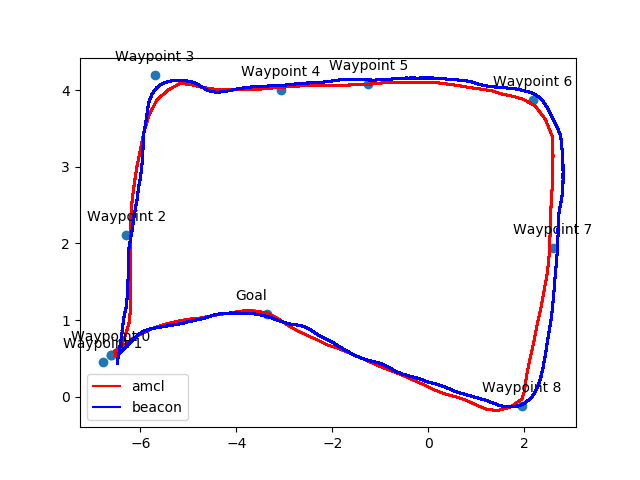
\includegraphics[scale=0.67]{Images/Chapter 5/plot_amclvsbeacon.png}
    \caption{Real time plot from beacon and AMCL pose }
    \label{fig:realtimeplot}
\end{figure}

However, the tool showed some shortcomings in robustness. The problem is mainly caused by the discontinuous signal the beacons send: it is sufficient for the mobile transmitter, placed on the robot, to have its reception field shielded for the modem to stop receiving signals on position tracking. The ultrasounds are in fact completely shielded when the robot and hedgehog are behind a column or physical object relative to the position of the modem transmitter. This is certainly critical with regard to the position plot, which is however an accessory and not a fundamental of testing, but even more so in the case of wanting to calculate the statistics between beacon and amcl pose. 


\subsection{Current Measure}
Another addition that was made to the testing module concerns the measurement of currents during navigation. It is indeed important to have an estimate of the current peaks that occur, the hypothetical and actual consumption of the robot. For this purpose, therefore, a programme was created which subscribes to the topic motor\_current in a callback and saves all data relating to the left and right motor. This is easily implementable due to the fact that the current message arrives in the form of a multi-array where at positions 0 and 1 are the current data for the left and right motor respectively. It is then possible by dividing by a factor of 10 to obtain the current values directly in ampere. From this data it was straightforward to calculate the data of the absorbed currents in A*h and consequently, by adding them up, estimate the absorption for 1 hour and 8 hours of use.
\begin{figure}[H]
    \centering
    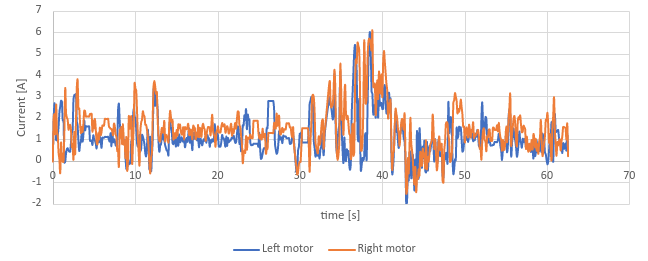
\includegraphics[scale=0.7]{Images/Chapter 5/motorcurrent.png}
    \caption{Left and Right Motor Current plot}
    \label{fig:motorcurrent}
\end{figure}
In figure \ref{fig:motorcurrent}, the plot of motor current is shown. These data were collected by driving the robot around a path that included the climbing and descending of a ramp. This particular path was a case of interest since an estimate of the battery consumption when dealing with ramps was needed. The peak of current values indeed correspond to the robot climbing the ramp. In the tables below are reported the computed estimate for a period of 1 and 8 hours.
\begin{table}[H]
\centering
\begin{tabular}{lll}
\textbf{Hypotetical Consumption} & \textbf{{[}Wh{]}} & \textbf{{[}Ah{]}} \\
\textbf{1 hours}                 & 124,0             & 2,6               \\
\textbf{8 hours}                 & 991,7             & 20,7             
\end{tabular}
\caption{Energy Consumption}
\label{tab:consumption}
\end{table}

\begin{table}[H]
\centering
\begin{tabular}{lc}
\textbf{Total Time {[}s{]}}          & 62,6  \\
\textbf{Avg. Absorption {[}Ah/s{]}}  & 0,001 \\
\textbf{Avg. Consumption {[}Wh/s{]}} & 0,034
\end{tabular}
\caption{Average Absorption and Consumption}
\label{tab:my-table}
\end{table}

The full description of the Python code can be found in Appendix \ref{ch:appB}.